
\pdfminorversion=4 % for acroread
%\documentclass[aspectratio=169,t,xcolor={usenames,dvipsnames}]{beamer}
\documentclass[aspectratio=169,t,handout,xcolor={usenames,dvipsnames}]{beamer}
\usepackage{../beamerstyle}
\usepackage{dsfont}
\usepackage{bm}
\usepackage[english]{babel}
\usepackage[utf8]{inputenc}
\usepackage{graphicx}
\usepackage{algorithm}
\usepackage[ruled,vlined,algo2e,linesnumbered]{algorithm2e}
%\usepackage[boxed,vlined]{algorithm2e}
\usepackage{hyperref}
\usepackage{booktabs}
\usepackage{mathtools}

\usepackage{amsmath,amssymb}
\usepackage{listings}
\lstset{frame=lines,framesep=3pt,numbers=left,numberblanklines=false,basicstyle=\ttfamily\small}

\usepackage{subfig}
\usepackage{multicol}
%\usepackage{appendixnumberbeamer}
%
\usepackage{tcolorbox}

\usepackage{pgfplots}
\usepackage{tikz}
\usetikzlibrary{trees} 
\usetikzlibrary{shapes.geometric}
\usetikzlibrary{positioning,shapes,shadows,arrows,calc,mindmap}
\usetikzlibrary{positioning,fadings,through}
\usetikzlibrary{decorations.pathreplacing}
\usetikzlibrary{intersections}
\usetikzlibrary{positioning,fit,calc,shadows,backgrounds}
\pgfdeclarelayer{background}
\pgfdeclarelayer{foreground}
\pgfsetlayers{background,main,foreground}
\tikzstyle{activity}=[rectangle, draw=black, rounded corners, text centered, text width=8em]
\tikzstyle{data}=[rectangle, draw=black, text centered, text width=8em]
\tikzstyle{myarrow}=[->, thick, draw=black]

% Define the layers to draw the diagram
\pgfdeclarelayer{background}
\pgfdeclarelayer{foreground}
\pgfsetlayers{background,main,foreground}

%\usepackage{listings}
%\lstset{numbers=left,
%  showstringspaces=false,
%  frame={tb},
%  captionpos=b,
%  lineskip=0pt,
%  basicstyle=\ttfamily,
%%  extendedchars=true,
%  stepnumber=1,
%  numberstyle=\small,
%  xleftmargin=1em,
%  breaklines
%}

 
\definecolor{blue}{RGB}{0, 74, 153}

\usetheme{Boadilla}
%\useinnertheme{rectangles}
\usecolortheme{whale}
\setbeamercolor{alerted text}{fg=blue}
\useoutertheme{infolines}
\setbeamertemplate{navigation symbols}{\vspace{-5pt}} % to lower the logo
\setbeamercolor{date in head/foot}{bg=white} % blue
\setbeamercolor{date in head/foot}{fg=white}
\setbeamercolor{author  in head/foot}{bg=white} %blue
\setbeamercolor{title in head/foot}{bg=white} % blue
\setbeamercolor{title}{fg=white, bg=blue}
\setbeamercolor{block title}{fg=white,bg=blue}
\setbeamercolor{block body}{bg=blue!10}
\setbeamercolor{frametitle}{fg=white, bg=blue}
\setbeamercovered{invisible}

\makeatletter
\setbeamertemplate{footline}
{
  \leavevmode%
  \hbox{%
  \begin{beamercolorbox}[wd=.333333\paperwidth,ht=2.25ex,dp=1ex,center]{author in head/foot}%
%    \usebeamerfont{author in head/foot}\insertshortauthor
  \end{beamercolorbox}%
  \begin{beamercolorbox}[wd=.333333\paperwidth,ht=2.25ex,dp=1ex,center]{title in head/foot}%
    \usebeamerfont{title in head/foot}\insertshorttitle
  \end{beamercolorbox}%
  \begin{beamercolorbox}[wd=.333333\paperwidth,ht=2.25ex,dp=1ex,right]{date in head/foot}%
    \usebeamerfont{date in head/foot}\insertshortdate{}\hspace*{2em}
%    \insertframenumber\hspace*{2ex} 
  \end{beamercolorbox}}%
  \vskip0pt%
}
\makeatother

%\pgfdeclareimage[height=1.2cm]{automl}{images/logos/automl.png}
%\pgfdeclareimage[height=1.2cm]{freiburg}{images/logos/freiburg}

%\logo{\pgfuseimage{freiburg}}

\renewcommand{\comment}[1]{
	\noindent
	%\vspace{0.25cm}
	{\color{red}{\textbf{TODO:} #1}}
	%\vspace{0.25cm}
}
\newcommand{\notefh}[1]{\textcolor{red}{\textbf{FH:} #1}}
\renewcommand{\comment}[1]{}
\newcommand{\hide}[1]{}
\newcommand{\cemph}[2]{\emph{\textcolor{#1}{#2}}}

\newcommand{\lit}[1]{{\footnotesize\color{black!60}[#1]}}

\newcommand{\litw}[1]{{\footnotesize\color{blue!20}[#1]}}


\newcommand{\myframe}[2]{\begin{frame}[c]{#1}#2\end{frame}}
\newcommand{\myframetop}[2]{\begin{frame}{#1}#2\end{frame}}
\newcommand{\myit}[1]{\begin{itemize}#1\end{itemize}}
\newcommand{\myblock}[2]{\begin{block}{#1}#2\end{block}}


\newcommand{\votepurple}[1]{\textcolor{Purple}{$\bigstar$}}
\newcommand{\voteyellow}[1]{\textcolor{Goldenrod}{$\bigstar$}}
\newcommand{\voteblue}[1]{\textcolor{RoyalBlue}{$\bigstar$}}
\newcommand{\votepink}[1]{\textcolor{Pink}{$\bigstar$}}

\newcommand{\diff}{\mathop{}\!\mathrm{d}}
\newcommand{\refstyle}[1]{{\small{\textcolor{gray}{#1}}}}
\newcommand{\hands}[0]{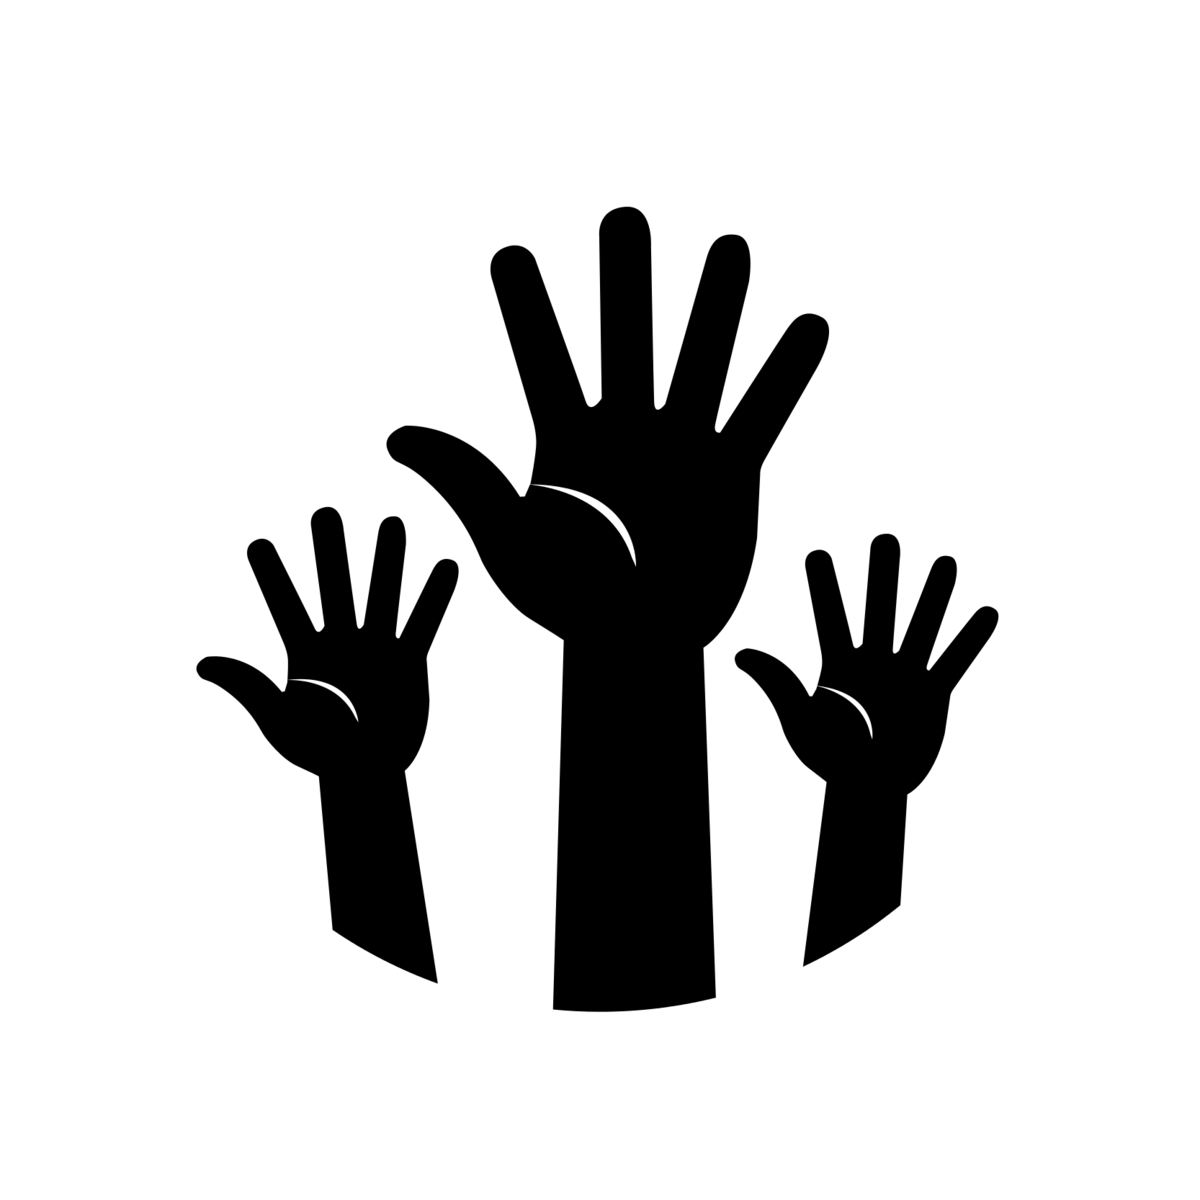
\includegraphics[height=1.5em]{images/hands}}
\newcommand{\transpose}[0]{{\textrm{\tiny{\sf{T}}}}}
\newcommand{\norm}{{\mathcal{N}}}
\newcommand{\cutoff}[0]{\kappa}
\newcommand{\instD}[0]{\dataset}
\newcommand{\insts}[0]{\mathcal{I}}
\newcommand{\inst}[0]{i}
\newcommand{\instI}[1]{i^{(#1)}}

% Iteration specific instance of variable/function/anything
% Introduced in the BO section, but moved up here to make it available within other macros
\newcommand{\iter}[2][\bocount]{{#2}^{(#1)}}

%--------HPO parameter macros-----------

% Parameter Configuration Space
\newcommand{\pcs}[0]{\pmb{\Lambda}}

% ???
\newcommand{\bx}[0]{\conf}

% Parameter Configuration
\newcommand{\conf}[0]{\pmb{\lambda}}

% Final Configuration
\newcommand{\finconf}[0]{\pmb{\hat{\lambda}}}

% Configuration corresponding to a given iteration -- better use \iter!
\newcommand{\confI}[1]{{\conf}^{(#1)}}

% Default Configuration
\newcommand{\defconf}[0]{{\conf}_{\text{def}}}

% Incumbent Configuration
\newcommand{\incumbent}[1][\bocount]{\iter[#1]{\finconf}}

% Optimal Configuration
\newcommand{\optconf}[0]{{\conf}^*}

% Configuration Space
\newcommand{\confs}[0]{\pcs}

%----------------------------------------

%\newcommand{\vlambda}[0]{\bm{\lambda}}
%\newcommand{\vLambda}[0]{\bm{\Lambda}}
\newcommand{\dataset}[0]{\mathcal{D}}
\newcommand{\datasets}[0]{\mathbf{D}}
\newcommand{\loss}[0]{L}
\newcommand{\risk}{\mathcal{R}}
\newcommand{\riske}{\mathcal{R}_{\text{emp}}}
\newcommand{\cost}[0]{c}
\newcommand{\costI}[1]{c^{(#1)}}

% Gaussian Process
\newcommand{\gp}{\mathcal{G}}
% Family of Objective Functions
\newcommand{\objF}{F}

%---------------BO Macros------------------

% BO loop counter
\newcommand{\bocount}{t}
% BO loop counter max, the counter runs from 1 to this value
\newcommand{\bobudget}{T}
% BO loop observation
\newcommand{\obs}[1][\conf]{\cost({#1})}
% BO loop observation space
\newcommand{\obsspace}{\mathcal{Y}}
% BO loop next observation
\newcommand{\bonextobs}{\obs[\iter{\conf}]}
% Acquisition Function, no args
\newcommand{\acq}{u}
% Standard Normal PDF
\newcommand{\pdf}{\phi}
% Standard Normal CDF
\newcommand{\cdf}{\Phi}
% Mean
\newcommand{\mean}{\mu}
% Standard Deviation
\newcommand{\stddev}{\sigma}
% Variance
\newcommand{\variance}{\sigma^2}
% Noise
\newcommand{\noise}{\nu}
% BO loop next selected sample
\newcommand{\bonextsample}{\confI{\bocount}}

% Single hyperparameter
\newcommand{\hyperparam}{\lambda}

% Single hyperparameter within a hyperparameter configuration
\newcommand{\hyperparami}[1][i]{{\hyperparam}_#1}

% Full definition of final configuration
\newcommand{\finconffull}{\incumbent[\bobudget]}

% Dataset
\newcommand{\datasetHPO}{{\dataset}_{HPO}}

% Dataset definition
\newcommand{\datasetHPOdef}{{\langle \bonextsample,\,\bonextobs \rangle}_{\bocount=1}^{\bobudget}}

% Double Display Fraction, forces large displays for everything in numerator and denominator
\newcommand\ddfrac[2]{\frac{\displaystyle #1}{\displaystyle #2}}

% Conditional Probability "Given That" Relation, source:https://tex.stackexchange.com/a/141685/205886
\newcommand\given[1][]{\:#1\vert\:}

% Expectation as a math operator
\DeclareMathOperator*{\E}{\mathbb{E}}

% Citation 
\newcommand{\source}[1]{
    \begin{flushright}
    	Source: \lit{#1}
    \end{flushright}
}
%-------------------------------------------

%Real numbers set
\newcommand{\realnum}{\mathbb{R}}
%Configuration space - do not use
%\newcommand{\configspace}{\Theta}
%Instances - do not use
%\newcommand{\instances}{\mathcal{I}}
%Expected value
\newcommand{\expectation}{\mathbb{E}}
%Kernel
\newcommand{\kernel}{\kappa}
%Constraint function
\newcommand{\constraintf}{c}
%Normal distribution
\newcommand{\normaldist}{\mathcal{N}}

% \renewcommand{\vec}[1]{\mathbf{#1}}
\newcommand{\hist}[0]{\dataset_{\text{Hist}}}
\newcommand{\param}[0]{p}
\newcommand{\algo}[0]{\mathcal{A}}
\newcommand{\algos}[0]{\mathbf{A}}
%\newcommand{\nn}[0]{N}
\newcommand{\feats}[0]{\mathcal{X}_{\text{meta}}}
\newcommand{\feat}[0]{\x_{\text{meta}}}
%\newcommand{\cluster}[0]{\vec{h}}
%\newcommand{\clusters}[0]{\vec{H}}
\newcommand{\perf}[0]{\mathbb{R}}
%\newcommand{\surro}[0]{\mathcal{S}}
\newcommand{\surro}[0]{\hat{\cost}}
\newcommand{\func}[0]{f}
\newcommand{\epm}[0]{\surro}
\newcommand{\portfolio}[0]{\mathbf{P}}
\newcommand{\schedule}[0]{\mathcal{S}}

% Machine Learning
\newcommand{\mdata}[0]{\dataset_{\text{meta}}}
\newcommand{\datasettrain}[0]{\dataset_{\text{train}}}
\newcommand{\datasetval}[0]{\dataset_{\text{val}}}
\newcommand{\datasettest}[0]{\dataset_{\text{test}}}
\newcommand{\x}[0]{\mathbf{x}}
\newcommand{\y}[0]{y}
\newcommand{\xI}[1]{\mathbf{x}^{(#1)}}
\newcommand{\yI}[1]{y^{(#1)}}
\newcommand{\fx}{f(\mathbf{x})}  % f(x), continuous prediction function
\newcommand{\Hspace}{\mathcal{H}} % hypothesis space where f is from
\newcommand{\fh}{\hat{f}}       % f hat, estimated prediction function

% Deep Learning
\newcommand{\weights}[0]{\theta}
\newcommand{\metaweights}[0]{\phi}


% reinforcement learning
\newcommand{\policies}[0]{\mathbf{\Pi}}
\newcommand{\policy}[0]{\pi}
\newcommand{\actionRL}[0]{a}
\newcommand{\stateRL}[0]{s}
\newcommand{\statesRL}[0]{\mathcal{S}}
\newcommand{\rewardRL}[0]{r}
\newcommand{\rewardfuncRL}[0]{\mathcal{R}}

\RestyleAlgo{algoruled}
\DontPrintSemicolon
\LinesNumbered
\SetAlgoVlined
\SetFuncSty{textsc}

\SetKwInOut{Input}{Input}
\SetKwInOut{Output}{Output}
\SetKw{Return}{return}

%\newcommand{\changed}[1]{{\color{red}#1}}

%\newcommand{\citeN}[1]{\citeauthor{#1}~(\citeyear{#1})}

\renewcommand{\vec}[1]{\mathbf{#1}}
\DeclareMathOperator*{\argmin}{arg\,min}
\DeclareMathOperator*{\argmax}{arg\,max}

%\newcommand{\aqme}{\textit{AQME}}
%\newcommand{\aslib}{\textit{ASlib}}
%\newcommand{\llama}{\textit{LLAMA}}
%\newcommand{\satzilla}{\textit{SATzilla}}
%\newcommand{\satzillaY}[1]{\textit{SATzilla'{#1}}}
%\newcommand{\snnap}{\textit{SNNAP}}
%\newcommand{\claspfolioTwo}{\textit{claspfolio~2}}
%\newcommand{\flexfolio}{\textit{FlexFolio}}
%\newcommand{\claspfolioOne}{\textit{claspfolio~1}}
%\newcommand{\isac}{\textit{ISAC}}
%\newcommand{\eisac}{\textit{EISAC}}
%\newcommand{\sss}{\textit{3S}}
%\newcommand{\sunny}{\textit{Sunny}}
%\newcommand{\ssspar}{\textit{3Spar}}
%\newcommand{\cshc}{\textit{CSHC}}
%\newcommand{\cshcpar}{\textit{CSHCpar}}
%\newcommand{\measp}{\textit{ME-ASP}}
%\newcommand{\aspeed}{\textit{aspeed}}
%\newcommand{\autofolio}{\textit{AutoFolio}}
%\newcommand{\cedalion}{\textit{Cedalion}}
\newcommand{\fanova}{\textit{fANOVA}}
\newcommand{\sbs}{\textit{SB}}
\newcommand{\oracle}{\textit{VBS}}

% like approaches
\newcommand{\claspfoliolike}[1]{\texttt{claspfolio-#1-like}}
\newcommand{\satzillalike}[1]{\texttt{SATzilla'#1-like}}
\newcommand{\isaclike}{\texttt{ISAC-like}}
\newcommand{\ssslike}{\texttt{3S-like}}
\newcommand{\measplike}{\texttt{ME-ASP-like}}

\newcommand{\irace}{\textit{I/F-race}}
\newcommand{\gga}{\textit{GGA}}
\newcommand{\smac}{\textit{SMAC}}
\newcommand{\paramils}{\textit{ParamILS}}
\newcommand{\spearmint}{\textit{Spearmint}}
\newcommand{\tpe}{\textit{TPE}}


\usepackage{pifont}
\newcommand{\itarrow}{\mbox{\Pisymbol{pzd}{229}}}
\newcommand{\ithook}{\mbox{\Pisymbol{pzd}{52}}}
\newcommand{\itcross}{\mbox{\Pisymbol{pzd}{56}}}
\newcommand{\ithand}{\mbox{\raisebox{-1pt}{\Pisymbol{pzd}{43}}}}

%\DeclareMathOperator*{\argmax}{arg\,max}

\newcommand{\ie}{{\it{}i.e.\/}}
\newcommand{\eg}{{\it{}e.g.\/}}
\newcommand{\cf}{{\it{}cf.\/}}
\newcommand{\wrt}{\mbox{w.r.t.}}
\newcommand{\vs}{{\it{}vs\/}}
\newcommand{\vsp}{{\it{}vs\/}}
\newcommand{\etc}{{\copyedit{etc.}}}
\newcommand{\etal}{{\it{}et al.\/}}

\newcommand{\pscProc}{{\bf procedure}}
\newcommand{\pscBegin}{{\bf begin}}
\newcommand{\pscEnd}{{\bf end}}
\newcommand{\pscEndIf}{{\bf endif}}
\newcommand{\pscFor}{{\bf for}}
\newcommand{\pscEach}{{\bf each}}
\newcommand{\pscThen}{{\bf then}}
\newcommand{\pscElse}{{\bf else}}
\newcommand{\pscWhile}{{\bf while}}
\newcommand{\pscIf}{{\bf if}}
\newcommand{\pscRepeat}{{\bf repeat}}
\newcommand{\pscUntil}{{\bf until}}
\newcommand{\pscWithProb}{{\bf with probability}}
\newcommand{\pscOtherwise}{{\bf otherwise}}
\newcommand{\pscDo}{{\bf do}}
\newcommand{\pscTo}{{\bf to}}
\newcommand{\pscOr}{{\bf or}}
\newcommand{\pscAnd}{{\bf and}}
\newcommand{\pscNot}{{\bf not}}
\newcommand{\pscFalse}{{\bf false}}
\newcommand{\pscEachElOf}{{\bf each element of}}
\newcommand{\pscReturn}{{\bf return}}

%\newcommand{\param}[1]{{\sl{}#1}}
\newcommand{\var}[1]{{\it{}#1}}
\newcommand{\cond}[1]{{\sf{}#1}}
%\newcommand{\state}[1]{{\sf{}#1}}
%\newcommand{\func}[1]{{\sl{}#1}}
\newcommand{\set}[1]{{\Bbb #1}}
%\newcommand{\inst}[1]{{\tt{}#1}}
\newcommand{\myurl}[1]{{\small\sf #1}}

\newcommand{\Nats}{{\Bbb N}}
\newcommand{\Reals}{{\Bbb R}}
\newcommand{\extset}[2]{\{#1 \; | \; #2\}}

\newcommand{\vbar}{$\,\;|$\hspace*{-1em}\raisebox{-0.3mm}{$\,\;\;|$}}
\newcommand{\vendbar}{\raisebox{+0.4mm}{$\,\;|$}}
\newcommand{\vend}{$\,\:\lfloor$}


\newcommand{\goleft}[2][.7]{\parbox[t]{#1\linewidth}{\strut\raggedright #2\strut}}
\newcommand{\rightimage}[2][.3]{\mbox{}\hfill\raisebox{1em-\height}[0pt][0pt]{\includegraphics[width=#1\linewidth]{#2}}\vspace*{-\baselineskip}}





\usepackage{multirow}


\title[AutoML: Risks]{AutoML: Evaluation} % week title
\subtitle{Background: Statistical Hypothesis Tests} % video title
\author[Marius Lindauer]{Bernd Bischl \and Frank Hutter \and Lars Kotthoff\newline \and \underline{Marius Lindauer} \and Joaquin Vanschoren}
\institute{}
\date{}

\newcommand\reffootnote[1]{%
	\begingroup
	\renewcommand\thefootnote{}\footnote{
		\tiny #1
		\vspace*{1em}}%
	\addtocounter{footnote}{-1}%
	\endgroup
}

% \AtBeginSection[] % Do nothing for \section*
% {
%   \begin{frame}{Outline}
%     \bigskip
%     \vfill
%     \tableofcontents[currentsection]
%   \end{frame}
% }

\begin{document}
	
	\maketitle
	
	%----------------------------------------------------------------------
	\begin{frame}[c]{Background: statistical hypothesis tests}
		
		\begin{itemize}
			\item When we have a lot of data, we need to summarize it
			\begin{itemize}
				\item But we already saw that summarization hides a lot of data
				%	  \item E.g., a single outlier might explain the difference in means
				\item Ideally, we want to draw high-level conclusions\\
				(e.g., ``A outperforms B on datasets of type X'')
			\end{itemize}
			
			\pause
			\bigskip
			
			\item Problem: we only have a finite number of observations
			\begin{itemize}
				\item Can we attribute observed performance differences to chance?
				\item Are we reasonably sure that a claim we make is reproducible?
				\item[$\leadsto$] Statistical tests can help
			\end{itemize}
			
			
		\end{itemize}
		
		\medskip
		
	\end{frame}
	%-----------------------------------------------------------------------
	%----------------------------------------------------------------------
	\begin{frame}[c]{Statistical hypothesis testing}
		
		\begin{enumerate}
			\item Define initial research hypothesis
			\pause
			\item Derive null $H_0$ and alternative $H_1$ hypothesis
			\begin{itemize}
				\item Alternative hypothesis should be your research hypothesis
			\end{itemize}
		\end{enumerate}	
		
	\end{frame}
	%-----------------------------------------------------------------------
	%----------------------------------------------------------------------
	\begin{frame}[c]{First example: Courtroom Tiral}
		
		\begin{itemize}
			\item A prosecutor tries to prove the guilt of the defendant
			\item $H_0$: The defendant is not guilty
				\begin{itemize}
					\item Accepted for the moment\\ (``not guilty as long as their guilt is not proven'') 
				\end{itemize}
			\item $H_1$: The defendant is guilty
				\begin{itemize}
					\item prosecutor hopes to support that
				\end{itemize}
			\pause
		\end{itemize}
		
		\medskip
		\pause
		\bigskip
		\centering
		\begin{tabular}{r|cc}
			\toprule
			& Truly not guilty 	& Truly guilty\\
			\hline
			Found not guilty 	& Acquittal & Type II Error\\
			Found guilty & Type I Error		& Conviction\\
			\bottomrule
		\end{tabular}	
		
		\bigskip
		$\leadsto$ We want to minimize Type I error!
		
	\end{frame}
	%-----------------------------------------------------------------------
	%----------------------------------------------------------------------
	\begin{frame}[c]{Statistical hypothesis testing (cont'd)}
		
		\begin{enumerate}
			\item Define initial research hypothesis
			\item Derive null $H_0$ and alternative $H_1$ hypothesis
			\begin{itemize}
				\item Alternative hypothesis should be your research hypothesis
			\end{itemize}
			\item Consider statistical assumptions
			\begin{itemize}
				\item E.g., is your data Gaussian distributed?
			\end{itemize}
			\pause
			\item Decide test and test statistic $T$
			\begin{itemize}
				\item The correct test depends on your statistical assumptions.
				\item Typically: if you use more assumptions, the test is more powerful\\ (i.e., less Type-I error)
			\end{itemize}
			\pause
			\item Decide significance level $\alpha$\\ (i.e., acceptable Type-I error to reject null hypothesis)
			\pause
			\item Compute observed $t_{obs}$ of test statistic $T$
			\item Calculate $p$-value given $t_{obs}$
			\begin{itemize}
				\item i.e., probability under the null hypothesis of sampling a test statistic as extreme as observed (probability of Type-I error)
			\end{itemize} 
			\pause
			\item If $p < \alpha$, reject null hypothesis in favor of alternative hypothesis
			\begin{itemize}
				\item If $p > \alpha$, it doesn't tell you anything about the null hypothesis!
			\end{itemize}
		\end{enumerate}	
		
	\end{frame}
	%-----------------------------------------------------------------------
	%----------------------------------------------------------------------
	\begin{frame}[c]{Second example for a statistical test}
		
		\begin{itemize}
			\item Claim: \alert{``the students in this course are more intelligent
				than average''}
			\bigskip
			\pause
			\item \alert{Null Hypothesis $H_0$}: $\mu=100$ ($\mu$ is the population
			mean of this class)
			\item \alert{Alternative Hypothesis $H_1$}: $\mu>100$ (\alert{one-sided} hypothesis)
			\bigskip
			\pause
			\item IQ values are known to be normally distributed with $X \sim
			\mathcal{N}(100,15)$
			\begin{itemize}
				\item$\to$ statistical assumption
			\end{itemize}
			% \\with mean $100$ and variance $15$: $X \sim \mathcal{N}(100,15)$
			
			\bigskip
			\pause
			
			\item Let's say we observed IQ values $x_i$ of 9 students in the class:
			\begin{itemize}
				\item $\{x_1,\dots,x_9\} = \{116, 128, 125, 119, 89, 99, 105, 116, 118\}$.
				\item The \alert{sample mean} is $\bar{x}=112.8$
				\item Does this data support the claim?
			\end{itemize}	
			
		\end{itemize}	
		
	\end{frame}
	%-----------------------------------------------------------------------
	%----------------------------------------------------------------------
	\begin{frame}[c]{Example continued}
		
		\begin{itemize}
			
			\item \alert{Distribution of the test statistic} 
			\begin{itemize}
				\item Under $H_0$, we know that each $x_i \sim \mathcal{N}(100,15)$
				\smallskip
				\item The \alert{test statistic} that we measure is the sample
				mean $\bar{x} = \frac{1}{9} \sum_{i=1}^9 x_i$
				%    \item[-] $\bar{x} \sim  \mathcal{N}(\mu=100,\sigma^2=15/\sqrt{n})=\mathcal{N}(100,5)$
				\bigskip
				\pause
				\item Under $H_0$, the distribution of $\bar{x}$ is
				$\mathcal{N}(100,15/\sqrt{9})$
				\begin{itemize}
					\item[-] Our observation $\bar{x}=112.8$ is quite extreme under that
					distribution
				\end{itemize}
			\end{itemize}	
		\end{itemize}
		
		\begin{center}
			%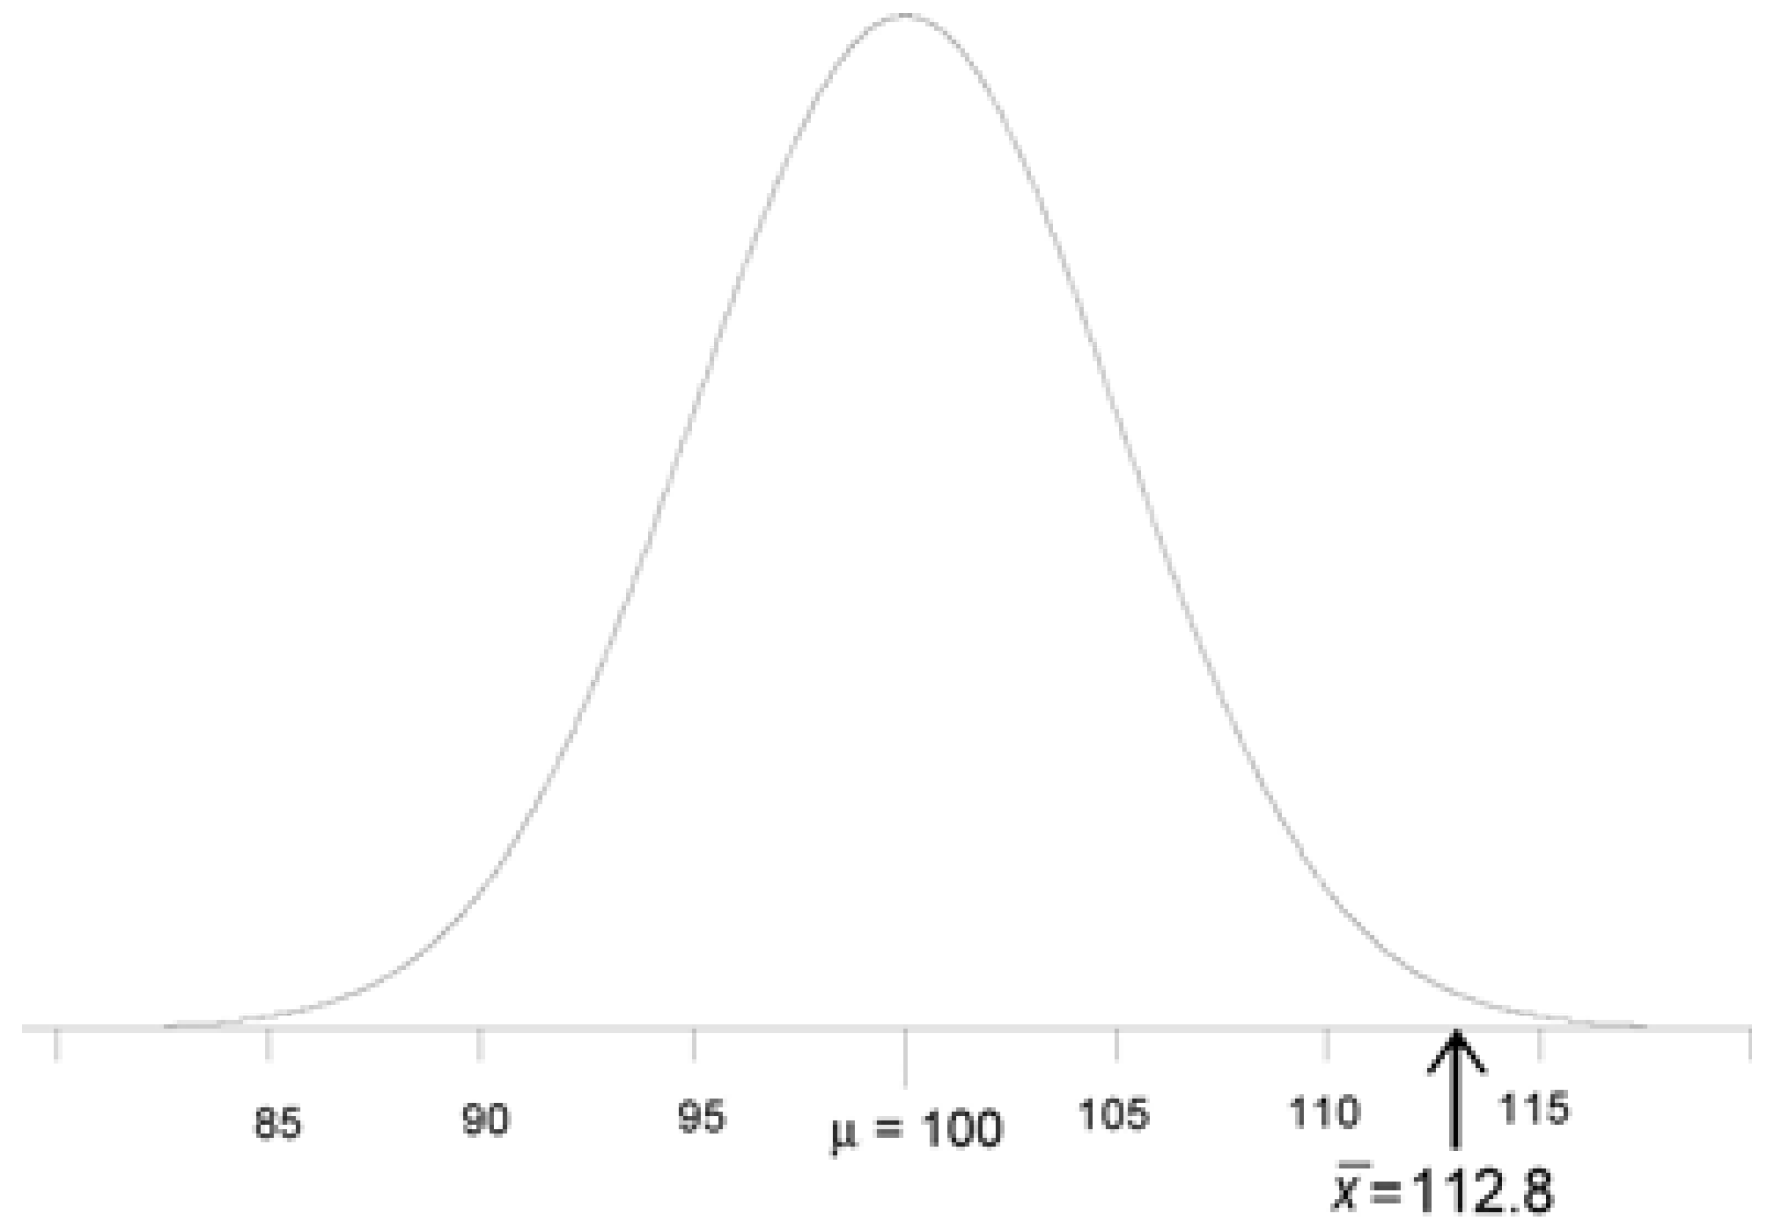
\includegraphics[height=3cm]{images/z_test_1.png}
			

\pgfmathdeclarefunction{gauss}{2}{%
	\pgfmathparse{1/(#2*sqrt(2*pi))*exp(-((x-#1)^2)/(2*#2^2))}%
}
\tikzstyle{myarrow}=[->, thick]
\begin{tikzpicture}
\begin{axis}[scale=0.75,
no markers, domain=82:118, samples=100,
axis lines*=left, xlabel=$IQ$,axis y line=none,
every axis x label/.style={at=(current axis.right of origin),anchor=west},
every x tick label/.append style={font=\scriptsize, yshift=0.5ex},
height=5cm, width=12cm,label style={font=\tiny},
xtick={80, 85, 90, 95, 100, 105, 110, 115, 120},
xticklabels={$80$, $85$, $90$, $95$, $100$, $105$, $110$, $115$, $120$},
ytick=\empty,
enlargelimits=false, clip=false, axis on top,
x=0.25cm, y=0.25cm/.004,
]
\addplot [thick,cyan!50!black] {gauss(100,15/sqrt(9))};
\coordinate (stat) at (axis cs:112.8,0.00325);
\coordinate (statlabel) at (axis cs:112.8,-.01);
\draw[myarrow, black!75] (statlabel) node [below, font=\scriptsize] {$\bar{x}=112.8$} -- (stat);
\end{axis}

\end{tikzpicture}
		\end{center}
		
	\end{frame}
	%-----------------------------------------------------------------------
	%----------------------------------------------------------------------
	\begin{frame}[c]{General principle}
		
		\vspace*{-0.2cm}
		\begin{center}
			%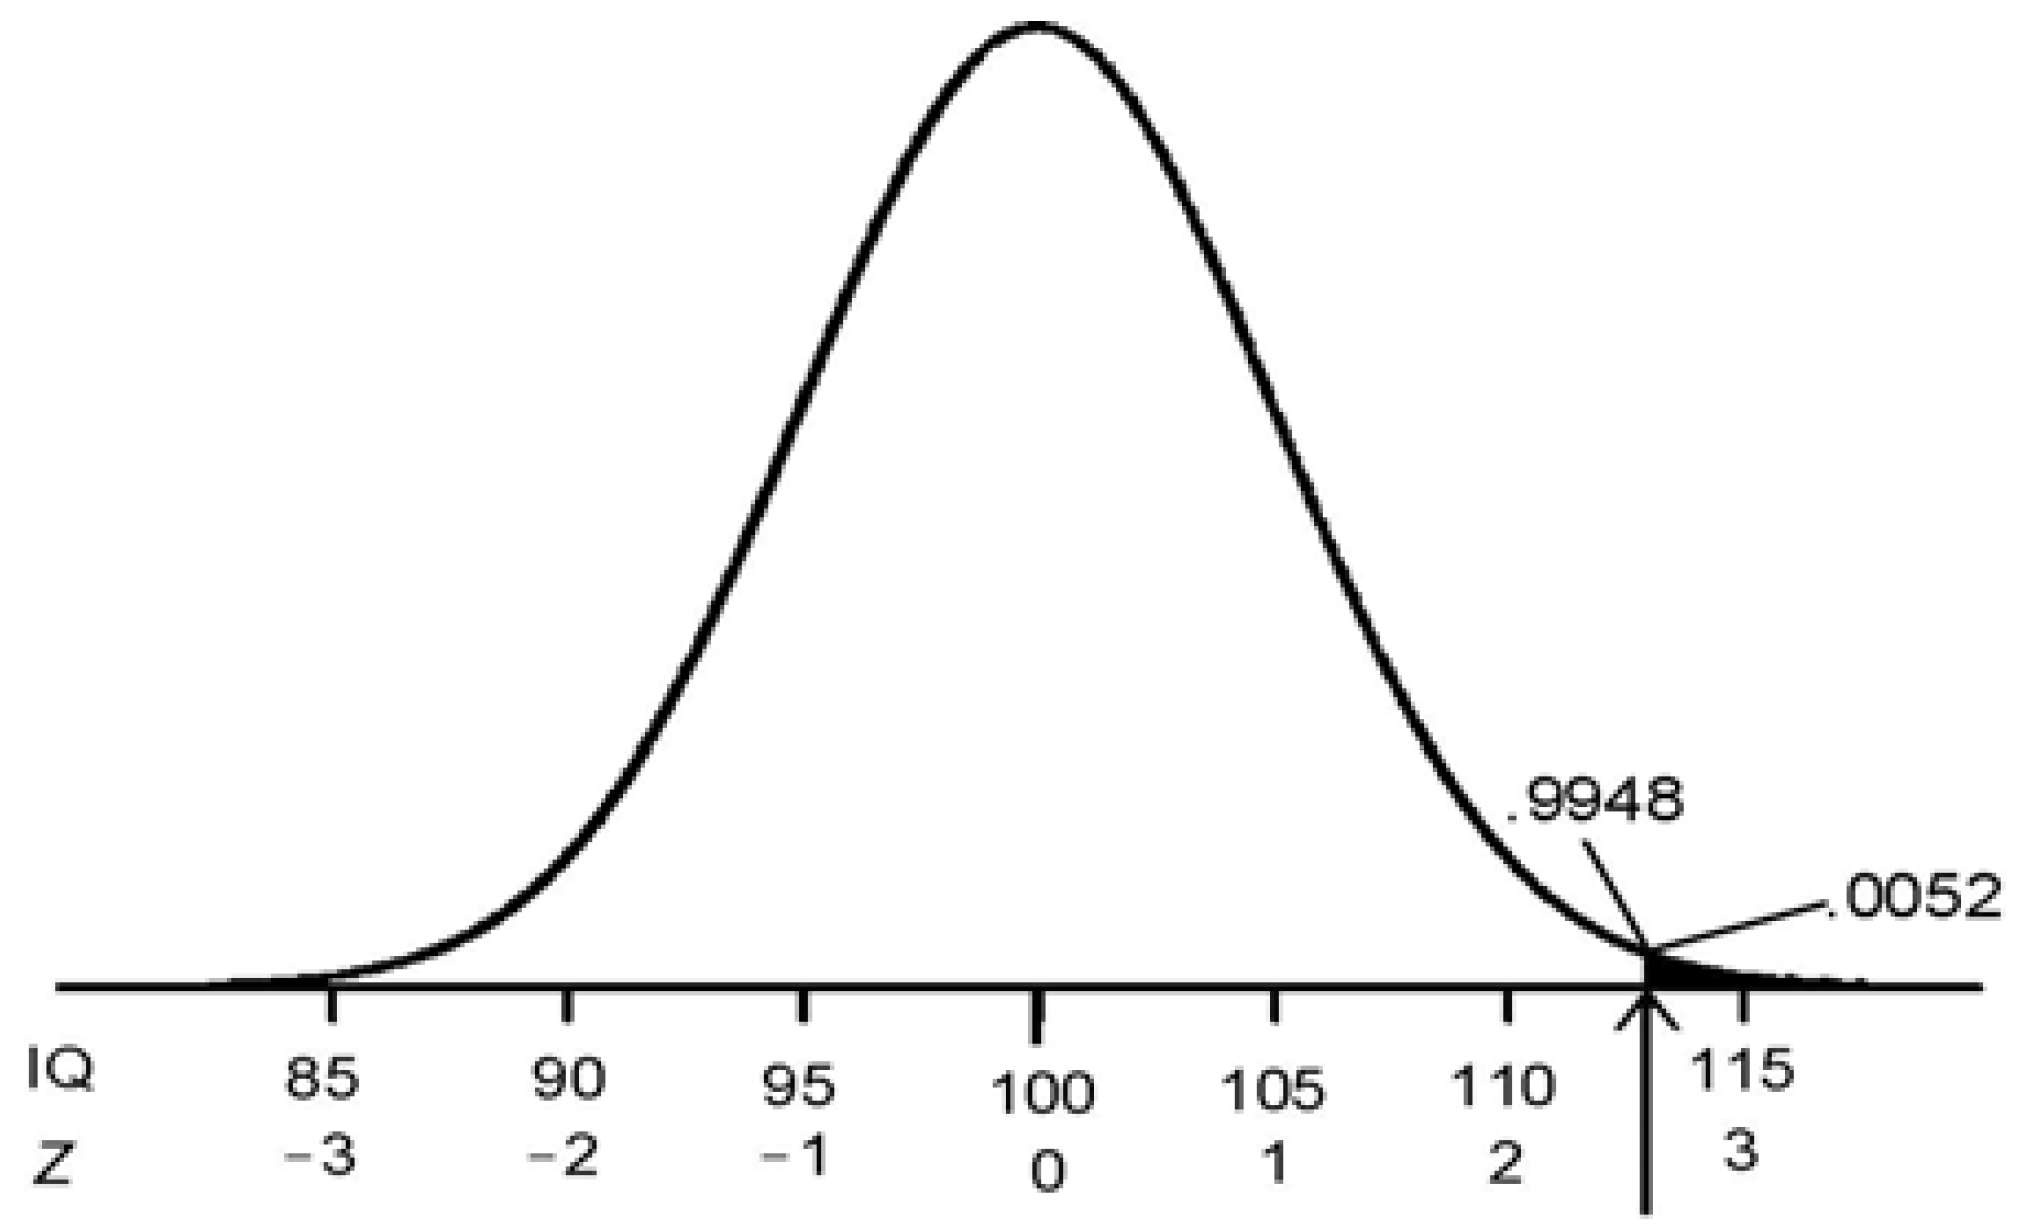
\includegraphics[height=3cm]{images/z_test_2.png}
			

\pgfmathdeclarefunction{gauss}{2}{%
	\pgfmathparse{1/(#2*sqrt(2*pi))*exp(-((x-#1)^2)/(2*#2^2))}%
}
\tikzstyle{myarrow}=[->, thick]
\begin{tikzpicture}
\begin{axis}[scale=0.525,
no markers, domain=82:118, samples=100,
axis lines*=left, xlabel=$IQ$,axis y line=none,
every axis x label/.style={at=(current axis.right of origin),anchor=west},
every x tick label/.append style={font=\scriptsize, yshift=0.5ex},
height=5cm, width=12cm,label style={font=\tiny},
xtick={80, 85, 90, 95, 100, 105, 110, 115, 120},
xticklabels={$80$, $85$, $90$, $95$, $100$, $105$, $110$, $115$, $120$},
ytick=\empty,
enlargelimits=false, clip=false, axis on top,
x=0.25cm, y=0.25cm/.004,
]
\addplot [fill=black!90, draw=none, domain=112.8:118] {gauss(100,15/sqrt(9))} \closedcycle;
\addplot [fill=black!10, draw=none, domain=82:112.8] {gauss(100,15/sqrt(9))} \closedcycle;
\addplot [thick,cyan!50!black] {gauss(100,15/sqrt(9))};
\coordinate (stat) at (axis cs:112.9,0.0035);
\coordinate (statlabelout) at (axis cs:115,0.0075);
\coordinate (statlabelin) at (axis cs:112,0.0125);
\draw[-, thin] (stat) -- (statlabelout) node[right,font=\tiny]{$.0052$};
\draw[-, thin, black!50] (stat) -- (statlabelin) node[above,font=\tiny]{$.9948$};
\end{axis}

\end{tikzpicture}
		\end{center}
		\vspace*{-0.2cm}
		
		\begin{itemize}
			\item Compare the test statistic (here: $\bar{x}$)\\to its sampling
			distribution under $H_0$
			\pause 
			\medskip
			\item \alert{P-value}: probability $p$ of observing values \alert{at least as extreme as $\bar{x}$}\\
			%  $\leadsto$ this is the %(computed through cumulative distribution function)
			\pause 
			\medskip
			\item Compare $p$ to pre-defined confidence level $\alpha$ (usually
			$\alpha=0.05$);\\\alert{if $p < \alpha$, reject $H_0$}
			\pause 
			\medskip
			\item With $\alpha = 0.01$, would we reject $H_0$ in this case?
		\end{itemize}
		
	\end{frame}
	%-----------------------------------------------------------------------
	%----------------------------------------------------------------------
	\begin{frame}[c]{Summary of example}
		
		\begin{itemize}
			\item We just used a so-called \alert{$Z$-test}
			\item $H_0$: $\mu=\mu_0$, $H_1$: $\mu>\mu_0$  
			\item Assumptions: $X \sim \mathcal{N}(\mu,\sigma^2)$ , with known $\mu$ and $\sigma^2$
			
			\medskip
			\pause
			\item \alert{Test statistic}: sample mean $\bar{x}$; evaluate under 
			$\mathcal{N}(\mu=\mu_0,s=\sigma^2/\sqrt{n})$
			\pause
			\smallskip
			\item Equivalent: compute the \alert{Z-statistic}: $Z = (\bar{x}-\mu_0)/s$
			and\\
			evaluate cumulative distribution $\Phi(Z)$ of $Z$
			under $\mathcal{N}(0,1)$
			\medskip
			\pause
			\begin{itemize}
				\item There are standard tables to look up $\Phi(Z)$ for different values of $Z$
				\item Nowadays, there are standard libraries to compute $\Phi(Z)$
			\end{itemize}
			
		\end{itemize}
		
	\end{frame}
	%-----------------------------------------------------------------------
	%----------------------------------------------------------------------
	\begin{frame}[c]{Two-sided tests}
		
		
		\vspace*{-0.2cm}
		\begin{center}
			%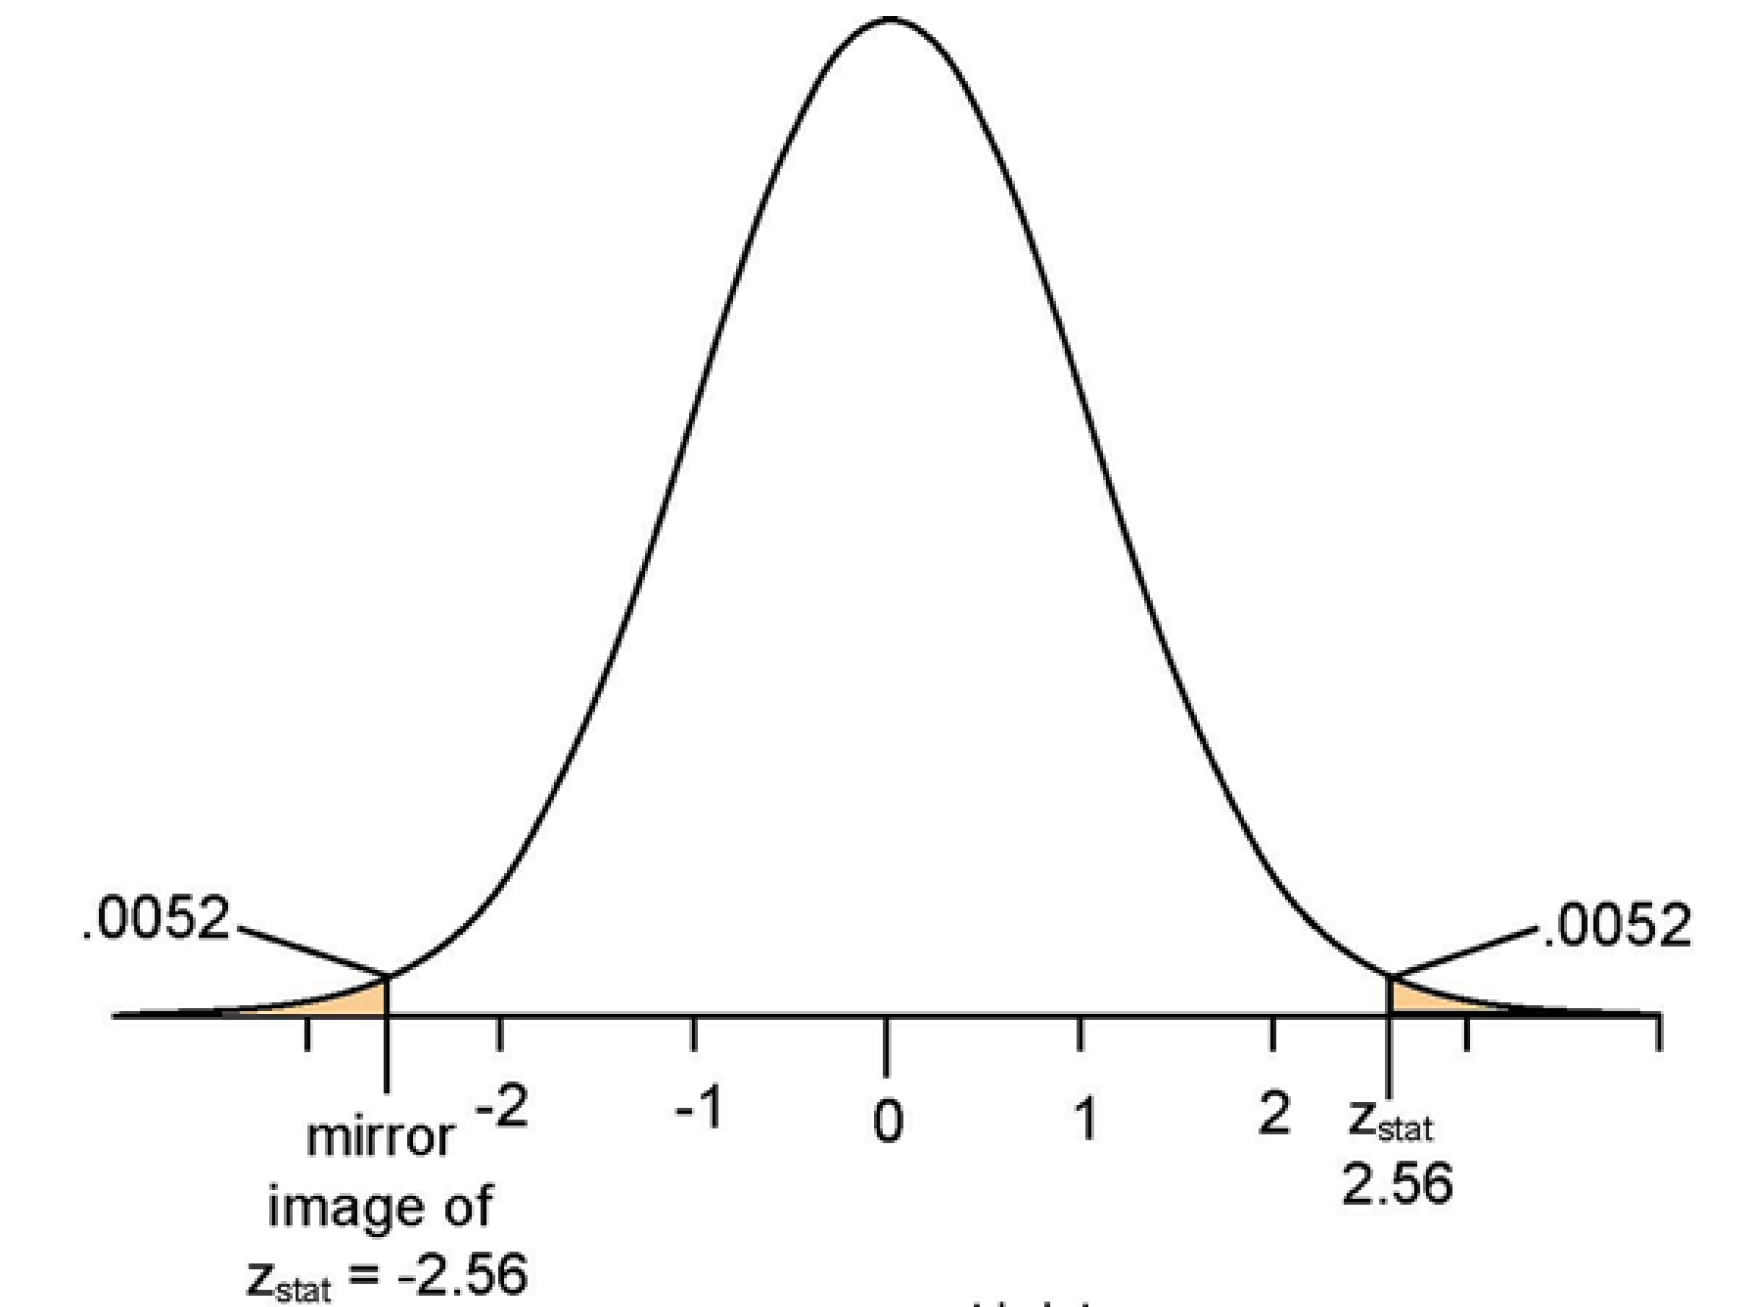
\includegraphics[height=3.5cm]{images/z_test_3.png}
			

\pgfmathdeclarefunction{gauss}{2}{%
	\pgfmathparse{1/(#2*sqrt(2*pi))*exp(-((x-#1)^2)/(2*#2^2))}%
}
\tikzstyle{myarrow}=[->, thick]
\begin{tikzpicture}
\begin{axis}[scale=0.525,
no markers, domain=82:118, samples=100,
axis lines*=left, xlabel=$IQ$,axis y line=none,
every axis x label/.style={at=(current axis.right of origin),anchor=west},
every x tick label/.append style={font=\scriptsize, yshift=0.5ex},
height=5cm, width=12cm,label style={font=\tiny},
xtick={80, 85, 90, 95, 100, 105, 110, 115, 120},
xticklabels={$80$, $85$, $90$, $95$, $100$, $105$, $110$, $115$, $120$},
ytick=\empty,
enlargelimits=false, clip=false, axis on top,
x=0.25cm, y=0.25cm/.004,
]
\addplot [fill=black!90, draw=none, domain=112.8:118] {gauss(100,15/sqrt(9))} \closedcycle;
\addplot [fill=black!90, draw=none, domain=82:87.2] {gauss(100,15/sqrt(9))} \closedcycle;
%\addplot [fill=black!10, draw=none, domain=82:112.8] {gauss(100,15/sqrt(9))} \closedcycle;
\addplot [thick,cyan!50!black] {gauss(100,15/sqrt(9))};
\coordinate (statright) at (axis cs:112.9,0.0035);
\coordinate (statleft) at (axis cs:87.2,0.0035);
\coordinate (statlabelright) at (axis cs:115,0.0075);
\coordinate (statlabelleft) at (axis cs:85,0.0075);
\draw[-, thin] (statleft) -- (statlabelleft) node[above,font=\tiny]{$.0052$};
\draw[-, thin, black] (statright) -- (statlabelright) node[above,font=\tiny]{$.0052$};
\end{axis}

\end{tikzpicture}
		\end{center}
		\vspace*{-0.2cm}
		
		\begin{itemize}
			\item Similar to one-sided tests, but testing for extreme values in both tails
			\item Example Z-test: two-sided alternative hypothesis $H_1$:
			$\mu \neq \mu_0$
			\pause
			\smallskip
			\item Compute $Z = (\bar{x}-\mu_0)/s$ as before
			\item Compute $p$-value as $p = 2\Phi(Z)$, to account for both tails
			\pause 
			\medskip
			\item With $\alpha = 0.01$, would we reject $H_0$ in this case? 
		\end{itemize}
		
	\end{frame}
	%-----------------------------------------------------------------------
	%----------------------------------------------------------------------
	\begin{frame}[c]{General points about statistical hypothesis tests}
		
		\begin{itemize}
			\item What if $p > \alpha$?
			\begin{itemize}
				\item \alert{Failure to reject $H_0$}
				\item \alert{We cannot conclude that we can accept $H_0$!}
			\end{itemize}
			
			
			\pause
			\bigskip
			\item Beware (i): most tests make some assumptions
			\begin{itemize}
				\item E.g., $Z$-test and popular $t$-test assume \alert{normality}
				\item Our data is often far from normally-distributed
				\begin{itemize}
					\item[$\leadsto$] E.g., exponential runtime distributions of optimizers
					\item[$\leadsto$] E.g., distribution of fitting a neural network\\ with different random seeds is not well studied
				\end{itemize}
			\end{itemize}
			\medskip
			\pause
			\item Beware (ii): if you use cross-validation, observations are not independent\\ (you cannot apply statistical tests that assume independence)
			%\begin{itemize}
			%	\item if you use bootstrap sampling, observations are independent
			%\end{itemize}
		\end{itemize}
		
	\end{frame}
	%-----------------------------------------------------------------------

	
\end{document}
